\documentclass[12pt,a4paper]{report}

% Encoding (important for pdfLaTeX)
\usepackage[utf8]{inputenc}
\usepackage[T1]{fontenc}

\usepackage{graphicx}
\usepackage{amsmath}
\usepackage{fancyhdr}
\usepackage{cite}
\usepackage{framed}
\usepackage{a4wide}
\usepackage{float}
\usepackage{multicol}
\usepackage{xpatch}
\usepackage{mathptmx}
\usepackage{geometry}
\usepackage{tocloft}

% Push TOC title and content upward aggressively
\setlength{\cftbeforetoctitleskip}{-3.5em}
\setlength{\cftaftertoctitleskip}{-0.5em}

% Reduce spacing between TOC entries
\setlength{\cftbeforechapskip}{0.2em}

\usepackage{listings}
\usepackage{color}
\usepackage{hyperref}
\usepackage{caption}
\usepackage{subcaption}

% Titlesec for normal-looking chapter headings
\usepackage{titlesec}

 \geometry{
 right=25mm,
 left=35mm,
 top=25mm,
 bottom=25mm,
 }

\makeatletter
\renewcommand{\cftdot}{}
\renewcommand{\cftchappresnum}{CHAPTER }
\renewcommand{\cftchapaftersnum}{:}
\renewcommand{\cftchapnumwidth}{6.5em}
\renewcommand\cftfigindent{0pt}
\renewcommand\cftfigpresnum{Figure\ }
\renewcommand\cftfigaftersnum{ : }
\renewcommand{\cftfignumwidth}{5.5em}
\renewcommand\cfttabpresnum{Table\ }
\renewcommand\cfttabaftersnum{ : }
\renewcommand{\cfttabnumwidth}{5em}
\makeatother

\titleformat{\chapter}[hang]
  {\normalfont\Large\bfseries} % format
  {\thechapter}{1em}{}          % label, sep, before-code
\titlespacing*{\chapter}{0pt}{*1.5}{*0.8}

\linespread{1.5}

% listings style for code snippets
\definecolor{lightgray}{gray}{0.95}
\lstset{
  basicstyle=\ttfamily\small,
  backgroundcolor=\color{lightgray},
  frame=single,
  breaklines=true,
  columns=fullflexible
}

\begin{document}

\begin{center}
{\Large \textbf{Context-Aware Music Intelligence System for Genre, Emotion, and Cognitive Compatibility Analysis}}\\
\vspace{0.5cm}

A PROJECT REPORT\\
FOR THE AWARD OF THE DEGREE\\
OF\\
BACHELOR OF TECHNOLOGY \\
IN\\
\textbf{Department of Computer Science and Engineering} \\
\vspace{1 cm}
Submitted by: \\

\textbf{Anurag Bandyopadhyay} \\
\textbf{(A91005222129)}\\
\vspace{1 cm}
Under the supervision of\\

Dr.Rekha Vig\\

\end{center}

\begin{center}
\begin{figure}[H]
    \centering
    \includegraphics[scale=0.4]{amity.jpg}
    \label{fig:logo}
\end{figure}
\textbf{DEPT. OF COMPUTER SCIENCE \& ENGINEERING}\\

Amity University Kolkata \\
Newtown, Kadampukur, West Bengal 700135\\
\textbf{December 2025}\\
\end{center}

\thispagestyle{empty}
\newpage
\pagenumbering{roman}
\begin{center}
%\vspace{1.5cm}
\textbf{DEPT. OF COMPUTER SCIENCE \& ENGINEERING}\\
Amity university Kolkata \\
Newtown, Kadampukur, West Bengal 700135\\
\end{center}

\begin{center}
\textbf{\underline{CANDIDATE’S DECLARATION}}\\
\addcontentsline{toc}{chapter}{Candidate’s Declaration}
\end{center}
\vspace{1.2cm}
I, Anurag Bandyopadhyay(A91005222129) student of B.Tech (Computer Science), hereby declare that the Project Dissertation titled ― “Context-Aware Music Intelligence System for Genre, Emotion, and Cognitive Compatibility Analysis” which is submitted by us to the Department of Engineering and Technology, Amity University, Kolkata in fulfillment of the requirement for awarding of the Bachelor of Technology degree, is not copied from any source without proper citation. This work has not previously formed the basis for the award of any Degree, Diploma, Fellowship or other similar title or recognition.

\noindent \begin{minipage}{4cm}
\begin{flushleft}
\vspace{5 cm}
                         
Place: Kolkata\\
Date: 11/12/2025\\

\end{flushleft} 
\end{minipage}
\hfill
\begin{minipage}{12cm}
\begin{flushright}                                      
\vspace{5 cm}
\vspace{1cm}
\textbf{Anurag Bandyopadhyay}
\vspace{0.2cm}
\textbf{(A91005222129)}\\
\vspace{0.2cm}


\end{flushright} 
\end{minipage}

\newpage
\begin{center}
%\vspace{1.5cm}
\textbf{DEPT. OF COMPUTER SCIENCE \& ENGINEERING}\\
Amity university Kolkata \\
Newtown, Kadampukur, West Bengal 700135\\
\end{center}

\vspace{2cm}
\begin{center}
 \textbf{\underline {CERTIFICATE}}
 \addcontentsline{toc}{chapter}{Certificate}
\end{center}
I hereby certify that the Project titled "Context-Aware Music Intelligence System for Genre, Emotion, and Cognitive Compatibility Analysis” which is submitted by Anurag Bandyopadhyay (A91005222129) for fulfillment of the requirements for awarding of the degree of Bachelor of Technology (B.tech) is a record of the project work carried out by the students under my guidance \& supervision. To the best of my knowledge, this work has not been submitted in any part or fulfillment for any Degree or Diploma to this University or elsewhere.

\noindent \begin{minipage}{4cm}
\begin{flushleft}
\vspace{1 cm}
                         
Place : Kolkata \\
Date : 11/12/2025 \\

\end{flushleft} 
\end{minipage}
\hfill
\begin{minipage}{10cm}
\begin{flushright}                                      
\vspace{2cm}
                         

\vspace{.8cm}
\textbf{Dr. Rekha Vig}\\
\textbf{(SUPERVISOR)}\\
Professor\\
Department of Engineering and Technology \\
Amity university Kolkata \\
Newtown, Kadampukur, West Bengal 700135\\
\end{flushright} 
\end{minipage}

\newpage
\begin{center}
 \textbf{\underline {ACKNOWLEDGEMENT}}
 \addcontentsline{toc}{chapter}{Acknowledgement}
\end{center}

The successful completion of any task is incomplete and meaningless without giving any due credit to the people who made it possible without which the project would not have been successful and would have existed in theory.

First and foremost, we are grateful to \textbf{Dr. Pronaya Bhattacharya}, HOD, Department of Engineering and technology, Amity University, and all other faculty members of our department for their constant guidance and support, constant motivation and sincere support and gratitude for this project work. We owe a lot of thanks to our supervisor, \textbf{Dr. Rekha Vig}, HOI, Department of Computer Science, Amity University for igniting and constantly motivating us and guiding us throughout the development and successful completion of this Major Project in undertaking this endeavor and challenge and also for being there whenever we needed her guidance or assistance.


We would also like to take this moment to show our thanks and gratitude to one and all, who indirectly or directly have given us their hand in this challenging task. We feel happy and joyful and content in expressing our vote of thanks to all those who have helped us and guided us in presenting this project work for our Major project. Last, but never least, we thank our well-wishers and parents for always being with us, in every sense and constantly supporting us in every possible sense whenever possible.



\vspace{2 cm}                       
\begin{flushright}
\textbf{Anurag Bandyopadhyay}
\textbf{(A91005222129)}\\
\end{flushright}
\vspace{0.3cm}

\newpage

% Abstract
\begin{center}
 \textbf{\underline {ABSTRACT}}
 \addcontentsline{toc}{chapter}{Abstract}
\end{center}

\vspace{0.5cm}

Music plays a significant role in influencing human emotions, concentration, relaxation, motivation, and cognitive behaviour. With the rapid growth of digital music platforms and intelligent recommendation systems, there is increasing demand for automated frameworks capable of understanding not only the structural properties of music, but also its emotional and contextual impact on listeners \cite{r1,r13}. Conventional music recommendation systems mainly rely on metadata, listening history, or collaborative filtering techniques, which often fail to analyze the intrinsic acoustic and psychological characteristics of music \cite{r11,r17}. Recent advancements in Artificial Intelligence, Deep Learning, Music Information Retrieval (MIR), and Music Emotion Recognition (MER) have enabled the development of intelligent audio analysis systems capable of extracting meaningful information directly from music signals \cite{r3,r4,r5,r14,r24,r25}.

This project presents a complete context-aware audio intelligence framework for music genre classification, emotion recognition, and cognitive compatibility analysis using Artificial Intelligence techniques. The proposed system integrates audio signal processing, deep learning, machine learning, contextual reasoning, and explainable AI into a unified real-time music analysis platform. Music genre classification is performed using Mel-spectrogram image representations and a Convolutional Neural Network (CNN), while emotion recognition is carried out using engineered acoustic features and a Random Forest classifier \cite{r3,r5,r9}. The system extracts multiple audio characteristics including MFCCs, chroma features, spectral contrast, tempo, energy, spectral centroid, spectral bandwidth, and zero-crossing rate to generate semantic music profiles and behavioral interpretations.

Unlike traditional music classification systems that only predict genre labels, the proposed framework evaluates whether a music track is contextually and cognitively suitable for a user’s current mood, activity, and desired mental state. A contextual intelligence engine analyzes emotional tone, stimulation level, rhythmic intensity, texture, and temporal emotional transitions to generate compatibility scores and cognitive metrics such as focus score, relaxation score, motivation score, emotional stability, and cognitive load. The framework also performs temporal emotion analysis by segmenting audio into smaller chunks and tracking emotional variation throughout the duration of the music signal.

A real-time interactive user interface is implemented using the Streamlit framework, enabling users to upload audio files and visualize genre predictions, emotional distributions, behavioral analysis, cognitive metrics, spectrograms, chromagrams, MFCCs, waveforms, and emotion timelines. Experimental evaluation demonstrates that the proposed hybrid AI framework provides reliable music understanding capabilities with strong practical applicability in intelligent recommendation systems, cognitive music analysis, personalized listening environments, and human-centered audio intelligence applications \cite{r4,r9,r14}.

\textbf{Keywords:} Music Information Retrieval, Deep Learning, Convolutional Neural Networks, Music Emotion Recognition, Audio Signal Processing, Context-Aware AI, Cognitive Music Analysis, Streamlit

\newpage

\tableofcontents
\newpage
\listoftables
\newpage
\listoffigures
\newpage

\pagenumbering{arabic}

\chapter{INTRODUCTION}

\section{Overview}

The rapid growth of digital music streaming platforms has led to a huge increase in the amount and variety of music available online. Modern music systems no longer depend only on playlists or genre labels, but increasingly use intelligent recommendation and analysis methods to understand music more effectively \cite{r1,r2}. Traditional systems mainly organize songs using metadata such as artist names, albums, or manually assigned genres. However, these approaches often fail to capture the emotional and behavioral impact music can have on listeners.

Music strongly influences human emotions, focus, stress levels, motivation, and relaxation. Properties such as tempo, energy, harmonic structure, and emotional tone can affect people differently depending on their mood or activity \cite{r3,r4}. Because of this, there is growing interest in systems that can analyze not just the genre or emotion of music, but also whether the music is suitable for a particular situation such as studying, meditation, exercise, relaxation, or sleep.

Recent progress in Artificial Intelligence (AI), Machine Learning (ML), Deep Learning (DL), and Music Information Retrieval (MIR) has improved the ability of computers to understand audio signals automatically \cite{r5,r6}. Convolutional Neural Networks (CNNs) perform well on spectrogram-based audio representations, while feature-based machine learning models can effectively recognize emotions using acoustic features such as MFCCs, chroma features, tempo, and spectral contrast \cite{r7,r8,r9,r10,r25,r26}.

This project presents a \textbf{Context-Aware Audio Intelligence System} capable of:

\begin{itemize}
    \item Music genre classification using CNN-based deep learning
    \item Emotion recognition using machine learning
    \item Temporal emotion analysis across audio segments
    \item Audio feature extraction and behavioral profiling
    \item Context-aware compatibility analysis
    \item Explainable visualization of music characteristics
\end{itemize}

Unlike conventional music classification systems that only predict labels, this system also evaluates whether a music track is suitable for the user’s current mood, activity, and mental state. It combines audio signal processing, deep learning, feature engineering, and contextual reasoning into a single framework for real-time music analysis.

The system uses two main AI approaches. A CNN model classifies music genres using Mel-spectrogram images, while a Random Forest classifier predicts emotions using extracted acoustic features. Their outputs are further analyzed using a contextual reasoning engine that studies compatibility between the music profile and the user’s current requirements.

An interactive Streamlit interface is used to support real-time analysis, emotion timelines, cognitive scoring, and visualization of audio features. The goal is to move beyond simple music classification and create a more human-centered music analysis system.

\section{Problem Formulation}

Most existing music analysis systems can predict genres or emotions separately, but they usually fail to answer an important real-world question:

\begin{center}
\textit{“Is this music suitable for my current emotional, cognitive, and situational context?”}
\end{center}

Traditional recommendation systems mainly rely on listening history, collaborative filtering, or metadata-based similarity methods \cite{r11}. These systems rarely analyze the actual acoustic behavior of music or its possible effect on the listener’s mental state.

Many existing systems also have several limitations:

\begin{itemize}
    \item Heavy dependence on metadata
    \item Lack of contextual reasoning
    \item Limited explainability
    \item No temporal emotion analysis
    \item No evaluation of cognitive suitability
\end{itemize}

To address these limitations, this project formulates the task as a multi-stage audio intelligence problem involving:

\begin{enumerate}
    \item Extraction of meaningful acoustic features from audio signals
    \item Genre classification using deep learning
    \item Emotion recognition using machine learning
    \item Temporal analysis of emotional transitions
    \item Behavioral interpretation of music characteristics
    \item Context-aware compatibility evaluation
\end{enumerate}

The aim is to transform traditional music classification into a more intelligent and context-aware analysis system.

\newpage

\section{Objectives}

The main objective of this project is to build a context-aware audio intelligence system capable of analyzing the structural, emotional, and behavioral properties of music using AI techniques.

The major objectives are:

\begin{itemize}

    \item To develop a CNN-based music genre classification model using Mel-spectrogram representations.

    \item To implement an emotion recognition system using acoustic features such as MFCCs, chroma features, spectral contrast, energy, and tempo.

    \item To perform temporal emotion analysis by segmenting audio into smaller chunks.

    \item To generate semantic music profiles using acoustic features and contextual rules.

    \item To evaluate whether music is suitable for activities such as studying, meditation, workouts, relaxation, and sleep preparation.

    \item To generate cognitive indicators such as focus score, relaxation score, motivation score, and cognitive load.

    \item To provide explainable outputs and visualizations for better interpretability.

    \item To build a real-time interactive interface using Streamlit.

\end{itemize}

\section{Motivation}

Music plays an important role in concentration, productivity, emotional regulation, and relaxation. People often select music based on preference or habit without knowing whether the music actually supports their intended mental or emotional state.

For example:

\begin{itemize}
    \item A student may listen to highly energetic music while studying, reducing focus.
    
    \item A stressed person may unknowingly choose emotionally intense music that increases mental fatigue.
    
    \item A person trying to relax or meditate may select music with high stimulation and rhythmic intensity.
\end{itemize}

Most music recommendation systems focus mainly on popularity, user history, or listening patterns rather than emotional or cognitive compatibility. This creates a gap between traditional recommendation systems and actual human-centered music understanding.

The motivation behind this project is to build an intelligent system that analyzes music beyond simple genre labels. By combining AI-based audio analysis with contextual reasoning, the system attempts to understand whether a music track matches the user’s current emotional and cognitive needs.

The project also explores the practical integration of Audio Signal Processing, Deep Learning, Machine Learning, Music Information Retrieval, Explainable AI into a single real-world application. 

\chapter{BACKGROUND}

\section{Music Feature Representations}

Audio signals are complex and continuously changing, which makes direct analysis difficult for machine learning models. Before classification, music signals are converted into representations that preserve important rhythmic, harmonic, and spectral information \cite{r13,r14}. Commonly used representations in Music Information Retrieval (MIR) include spectrograms, Mel-spectrograms, MFCCs, and chroma features.

Spectrograms represent frequency variation over time using Short-Time Fourier Transform (STFT), while Mel-spectrograms use the Mel frequency scale to better match human auditory perception \cite{r3,r5,r14}. MFCCs are widely used for capturing timbral properties of audio, especially in speech and emotion recognition tasks \cite{r9,r14}. Chroma features capture harmonic information by mapping spectral energy into musical pitch classes \cite{r2,r11,r12}.

This system mainly uses Mel-spectrograms for genre classification because they preserve important time--frequency patterns and work well with CNN-based models. For emotion recognition and contextual analysis, features such as MFCCs, chroma features, tempo, energy, spectral centroid, spectral bandwidth, and zero-crossing rate are extracted directly from audio signals.

Combining image-based and feature-based representations helps the system analyze both the structural and emotional characteristics of music effectively.

\section{Deep Learning for Audio}

Deep learning has significantly improved modern audio analysis systems by allowing models to learn features directly from data instead of depending only on handcrafted descriptors \cite{r13,r14}. Earlier music classification approaches mainly used manually designed features with shallow machine learning algorithms, which often struggled to generalize across different music styles \cite{r1,r17}.

Recent studies show that Convolutional Neural Networks (CNNs) perform well on spectrogram-based audio representations \cite{r3,r4,r5}. Since Mel-spectrograms behave similarly to images, CNNs can learn local patterns related to rhythm, texture, and frequency variations in music signals. Pooling operations further reduce dimensionality while preserving important information.

In this project, Mel-spectrogram images generated from segmented audio samples are used as inputs to a CNN model for genre classification. Along with deep learning, a Random Forest classifier is used for emotion recognition using extracted acoustic features. This combination provides both effective feature learning and interpretable prediction behaviour.

\section{Related Work}

Music analysis has remained an important research area in Music Information Retrieval for many years. Early work by Tzanetakis and Cook introduced music genre classification using handcrafted rhythmic, pitch-based, and timbral features with traditional machine learning classifiers \cite{r1}. Although influential, these methods depended heavily on manual feature engineering \cite{r17}.

Later research shifted towards deep learning-based audio analysis. Humphrey et al.\ showed that deep architectures can automatically learn more effective audio representations than handcrafted descriptors \cite{r7}. Choi et al.\ demonstrated that CNNs trained on spectrogram-based representations achieve strong performance in large-scale music classification tasks \cite{r3}. Hershey et al.\ further validated the effectiveness of deep CNN architectures for audio classification across multiple datasets \cite{r4}.

Recent work has also focused on music emotion recognition using features such as MFCCs, tempo, spectral descriptors, and energy combined with machine learning models including Random Forest classifiers \cite{r9,r14,r24,r25,r26}. More recent studies explore context-aware music analysis, explainable music intelligence, and emotionally adaptive recommendation systems \cite{r27,r28}.

This project combines genre classification, emotion recognition, temporal emotion analysis, contextual reasoning, and cognitive compatibility evaluation into a single music intelligence framework.

\chapter{SYSTEM ANALYSIS}

\section{Functional Requirements}

The system is designed to perform intelligent music analysis through real-time audio processing and contextual reasoning. Users should be able to upload audio files in formats such as WAV and MP3 through a Streamlit-based interface \cite{r21}. The uploaded audio is automatically preprocessed, segmented, and analyzed using audio signal processing techniques \cite{r13,r14}.

Mel-spectrograms generated from audio segments are used for genre classification through a CNN model \cite{r3,r5}. At the same time, acoustic features including MFCCs, chroma features, tempo, spectral contrast, energy, spectral centroid, spectral bandwidth, and zero-crossing rate are extracted for emotion recognition and behavioral analysis \cite{r9,r14}.

The system also performs temporal emotion analysis across multiple audio segments and generates semantic music profiles describing emotional tone, stimulation level, texture, and focus suitability. Based on the user’s mood, activity, and desired outcome, the contextual reasoning module evaluates music compatibility and generates cognitive indicators such as focus score, relaxation score, motivation score, emotional stability, and cognitive load.

The final predictions, visualizations, emotion timelines, and behavioral interpretations are displayed through an interactive dashboard.

\section{Non-functional Requirements}

The system should provide a lightweight and responsive interface using Streamlit for smooth interaction and real-time visualization \cite{r21}. The trained machine learning and deep learning models must load reliably during inference while maintaining low latency on CPU-based systems \cite{r4,r14,r20}.

The architecture is designed to remain modular so that future datasets, models, and contextual reasoning techniques can be integrated easily. The implementation should also remain compatible with standard Python libraries such as PyTorch, Librosa, Scikit-learn, NumPy, and Matplotlib.

In addition to prediction accuracy, the system should generate interpretable outputs and visual explanations to improve transparency and usability.

\section{High-level Architecture}

\begin{figure}[H]
    \centering
    \hspace{-0.84cm}
    \includegraphics[width=1.05\textwidth,height=0.92\textheight,keepaspectratio]{high_level_architecture.png}
    \caption{High-level architecture of the context-aware audio intelligence system.}
    \label{fig:architecture}
\end{figure}

\chapter{DATASET}

\begin{multicols}{2}

\section*{Genre Classes}

The genre classification model is trained on five music categories: Classical, Hip-Hop, Jazz, Pop, and Rock. These genres were selected because they differ clearly in rhythm, instrumentation, harmonic structure, and spectral behaviour, helping the CNN learn distinct time--frequency patterns effectively.

\columnbreak

\section*{Emotion Classes}

The emotion recognition pipeline supports four emotion categories: Calm, Happy, Sad, and Angry. These emotions represent clearly distinguishable acoustic and psychological patterns commonly used in music emotion recognition research.

\end{multicols}

\section*{Dataset Structure}

Separate datasets are used for genre classification and emotion recognition. Genre classification uses Mel-spectrogram image datasets generated from audio recordings, while the emotion pipeline uses labeled audio files for direct acoustic feature extraction.

\begin{verbatim}
dataset/
    genre/
        classical/
        hiphop/
        jazz/
        pop/
        rock/

    images/
        classical/
        hiphop/
        jazz/
        pop/
        rock/
    
    emotion/
        calm/
        happy/
        sad/
        angry/
\end{verbatim}

Audio files are first converted into Mel-spectrogram images using \texttt{audio\_to\_img.py}. These spectrogram images are organized into genre-wise folders for CNN training. For emotion recognition, audio files are mapped to emotion labels through CSV-based preprocessing.

\section{Data Preprocessing}

Before training and inference, audio signals undergo preprocessing to improve consistency and learning stability \cite{r3,r5,r14}. The pipeline includes normalization, silence removal, segmentation, spectrogram generation, image preprocessing, and acoustic feature extraction.

Audio files are loaded using Librosa with a fixed sampling rate of 22050 Hz. Silence and low-energy regions are trimmed to remove unnecessary segments from recordings. Long audio tracks are then divided into smaller chunks to improve dataset diversity and allow temporal analysis.

For genre classification, 10-second audio segments are converted into Mel-spectrograms using Librosa with 128 Mel bands, FFT window size 2048, and hop length 512. The spectrograms are transformed into logarithmic decibel scale and stored as PNG images for CNN training.

All spectrogram images are resized to \(128 \times 128\) before training. Tensor normalization and light augmentation techniques such as small rotations, horizontal flipping, and affine transformations are applied to improve generalization.

For emotion recognition and contextual analysis, acoustic features including MFCCs, chroma features, spectral contrast, tempo, energy, spectral centroid, spectral bandwidth, and zero-crossing rate are extracted directly from audio signals. These features form the input feature vector used by the Random Forest classifier.

\section{Dataset Preparation Workflow}

\begin{figure}[H]
    \centering
    \includegraphics[width=0.92\textwidth]{dataset_pipeline.png}
    \caption{Dataset preparation and preprocessing workflow.}
    \label{fig:datasetworkflow}
\end{figure}

\chapter{FEATURE EXTRACTION}

\section{Mel-spectrogram Generation}

For genre classification, audio signals are converted into Mel-spectrogram images which are later used as inputs to the CNN model. Mel-spectrograms preserve important rhythmic, harmonic, and frequency information while representing audio in an image-like format suitable for deep learning \cite{r3,r5,r14}.

The spectrogram generation process is implemented using \texttt{audio\_to\_img.py}. Audio files are loaded using Librosa with a sampling rate of 22050 Hz, normalized, trimmed, and divided into smaller segments before spectrogram generation. Instead of generating a single spectrogram for the entire track, multiple spectrograms are created from different temporal regions of the audio signal to improve dataset diversity and model robustness.

The preprocessing pipeline uses a sampling rate of 22050 Hz, FFT window size 2048, hop length 512, and 128 Mel bands. The generated spectrograms are converted into logarithmic decibel scale and stored as PNG images before resizing to \(128 \times 128\) for CNN training.

\begin{lstlisting}
# snippet from audio_to_img.py

mel = librosa.feature.melspectrogram(
    y=y_segment,
    sr=sr,
    n_mels=128,
    n_fft=2048,
    hop_length=512
)

log_mel = librosa.power_to_db(
    mel,
    ref=np.max
)
\end{lstlisting}

\section{Chunk-wise Audio Processing}

The system processes audio in smaller chunks instead of using the entire music track as a single input sample. This improves robustness and allows temporal analysis across different parts of the signal.

For genre classification, multiple 10-second segments are converted into Mel-spectrograms and passed individually through the CNN model. Final predictions are generated using majority voting across segment-level outputs.

For emotion recognition, audio is divided into 7-second chunks before feature extraction. This helps the system analyze emotional variation throughout the music track and generate emotion timelines instead of static predictions.

Chunk-wise processing improves dataset diversity, reduces sensitivity to local noise, and produces more stable predictions.

\section{Acoustic Feature Extraction}

For emotion recognition and contextual analysis, several acoustic features are extracted directly from audio signals using the \texttt{audio\_feature.py} module. These features capture rhythmic, harmonic, spectral, and timbral characteristics of music.

The extracted features include MFCCs, chroma features, spectral contrast, tempo, RMS energy, spectral centroid, spectral bandwidth, and zero-crossing rate.

MFCCs capture timbral properties, chroma features represent harmonic structure, while spectral descriptors describe brightness and texture. Tempo and energy help estimate rhythmic intensity and emotional behaviour. These features are combined into a numerical feature vector used for Random Forest-based emotion classification and contextual analysis.

\begin{lstlisting}
# snippet from audio_feature.py

mfcc = np.mean(
    librosa.feature.mfcc(
        y=y,
        sr=sr,
        n_mfcc=25
    ),
    axis=1
)

tempo, _ = librosa.beat.beat_track(
    y=y,
    sr=sr
)
\end{lstlisting}

\section{Semantic Music Profiling}

After feature extraction, the system generates a semantic music profile describing behavioral and cognitive properties of the music signal. Numerical features are converted into interpretable descriptors such as tempo type, energy level, stimulation intensity, texture, and focus suitability.

The profiling engine uses rule-based thresholds to classify music behaviour. For example, tempo may be categorized as slow, medium, or fast, while energy can be classified as low, moderate, or high. These descriptors are later used for contextual compatibility analysis.

\begin{lstlisting}
# snippet from music_profile.py

if tempo_type == "fast" and \
   energy_level == "high":
    return "intense"

if tempo_type == "slow" and \
   energy_level == "low":
    return "calm"
\end{lstlisting}

This profiling stage helps the system move beyond simple classification and perform higher-level behavioral interpretation of music signals.

\chapter{MODEL DESIGN AND TRAINING}

\section{Genre Classification Model}

Music genre classification is implemented using a Convolutional Neural Network (CNN) trained on Mel-spectrogram images generated from audio signals. CNNs are well suited for spectrogram-based audio analysis because they can learn local rhythmic and frequency patterns directly from image-like representations \cite{r3,r4,r5,r14}.

The model is implemented in \texttt{train\_model.py} using PyTorch. The architecture contains three convolutional blocks with 32, 64, and 128 filters respectively. Each block includes convolution, batch normalization, ReLU activation, and max-pooling operations for hierarchical feature extraction.

Batch normalization improves training stability while max-pooling reduces spatial dimensions and computational complexity \cite{r10,r15}. Adaptive Average Pooling is applied before the fully connected layers to reduce parameter count and improve robustness against spectrogram variations. A dropout layer with rate 0.4 is used to reduce overfitting.

\begin{lstlisting}
# CNN architecture snippet

self.conv = nn.Sequential(

    nn.Conv2d(3, 32, 3, padding=1),
    nn.BatchNorm2d(32),
    nn.ReLU(),
    nn.MaxPool2d(2),

    nn.Conv2d(32, 64, 3, padding=1),
    nn.BatchNorm2d(64),
    nn.ReLU(),
    nn.MaxPool2d(2),

    nn.Conv2d(64, 128, 3, padding=1),
    nn.BatchNorm2d(128),
    nn.ReLU(),
    nn.MaxPool2d(2)
)
\end{lstlisting}

\begin{figure}[H]
    \centering
    \includegraphics[width=0.9\textwidth]{cnn_architecture.png}
    \caption{CNN architecture used for genre classification.}
    \label{fig:cnnarchitecture}
\end{figure}

The model provides good classification performance while remaining lightweight enough for CPU-based inference.

\section{Emotion Recognition Model}

Emotion recognition is implemented using a Random Forest classifier trained on extracted acoustic features instead of spectrogram images. The feature vector contains MFCCs, chroma features, spectral contrast, tempo, RMS energy, spectral centroid, spectral bandwidth, and zero-crossing rate.

These features capture rhythmic, harmonic, timbral, and spectral characteristics of music signals. Random Forest was selected because of its strong performance on structured numerical data and its ability to handle non-linear decision boundaries efficiently \cite{r9,r14,r23}.

Audio is divided into 7-second chunks before feature extraction, allowing the system to perform temporal emotion analysis across different parts of the music signal.

\begin{lstlisting}
# Random Forest configuration

model = RandomForestClassifier(
    n_estimators=300,
    max_depth=20,
    max_features="sqrt",
    min_samples_split=5,
    min_samples_leaf=2,
    class_weight="balanced"
)
\end{lstlisting}

The trained model is stored as \texttt{emotion\_model.pkl} for real-time inference.

\section{Contextual Intelligence Framework}

Most music analysis systems only predict genre or emotion labels. This project additionally evaluates whether the selected music is suitable for the user’s current mood, activity, and desired mental state.

The contextual intelligence module combines acoustic feature analysis, emotion recognition, semantic profiling, and rule-based reasoning to generate compatibility scores and behavioral interpretations.

Extracted features are converted into semantic descriptors such as slow/fast tempo, low/high energy, smooth/noisy texture, and calm/intense stimulation. These descriptors are then compared with user context including mood, activity, and cognitive goals.

For example, highly intense music may reduce concentration during studying, while calm low-energy music may support relaxation or meditation. Similarly, fast energetic tracks may positively support workout environments.

The system generates compatibility scores, contextual recommendations, emotional stability analysis, and cognitive metrics such as focus score, relaxation score, and motivation score.

\begin{figure}[H]
    \centering
    \includegraphics[width=0.9\textwidth]{contextual_pipeline.png}
    \caption{Contextual intelligence workflow of the proposed system.}
    \label{fig:contextualpipeline}
\end{figure}

\section{Training Configuration}

All Mel-spectrogram images are resized to \(128 \times 128\) before training. The CNN uses a batch size of 16 and is trained for 20 epochs using the Adam optimizer with cross-entropy loss.

To improve generalization, augmentation techniques such as horizontal flipping, small rotations, and affine transformations are applied during training. A \texttt{ReduceLROnPlateau} scheduler dynamically lowers the learning rate when validation performance stops improving.

The framework also supports automatic hardware-aware execution using Apple MPS acceleration when available, otherwise falling back to CPU execution.

\begin{lstlisting}
device = torch.device(
    "mps" if torch.backends.mps.is_available()
    else "cpu"
)
\end{lstlisting}

The trained models are stored as:

\begin{itemize}
    \item \texttt{models/model.pth}
    \item \texttt{models/emotion\_model.pkl}
\end{itemize}

\section{Inference Workflow}

During inference, uploaded audio files are first segmented into smaller chunks. For genre classification, multiple 10-second segments are converted into Mel-spectrograms and classified independently by the CNN. Final predictions are generated using majority voting across all segments.

For emotion recognition, 7-second chunks are analyzed separately to generate temporal emotion timelines. The contextual intelligence module then combines genre predictions, emotional analysis, and semantic descriptors to generate behavioral interpretations and compatibility analysis.

The final output includes genre prediction, overall emotion, emotion timelines, cognitive scores, contextual recommendations, and explainable visualizations.  

\chapter{IMPLEMENTATION}

\section{System Implementation}

The system is implemented in Python using PyTorch for CNN-based genre classification, Scikit-learn for Random Forest emotion recognition, Librosa for audio processing, Streamlit for the web interface, and Matplotlib for visualizations. NumPy and Pandas are used for numerical operations and structured data handling.

The implementation pipeline includes audio upload, preprocessing, segmentation, feature extraction, Mel-spectrogram generation, genre prediction, emotion recognition, contextual analysis, and explainable visualization generation.

Unlike traditional recommendation systems that mainly depend on listening history or collaborative filtering, this framework performs direct audio-based reasoning using acoustic features and emotional analysis. This allows the system to generate contextual and interpretable outputs instead of static recommendations.

\section{Streamlit-Based User Interface}

The user interface is developed using Streamlit to provide a real-time music analysis dashboard. Users can upload audio files, specify contextual information, and visualize genre predictions, emotional analysis, cognitive scores, and audio feature visualizations.

The dashboard displays genre prediction, emotion timelines, behavioral analysis, cognitive compatibility scores, spectrograms, MFCC plots, chromagrams, waveforms, and explainable reasoning outputs.

User context is collected through mood, activity, and desired outcome selections, which are later used by the contextual intelligence engine during compatibility evaluation.

\begin{lstlisting}
user_mood = st.selectbox(
    "Current Mood",
    ["stressed", "sad", "calm",
     "happy", "motivated", "tired"]
)

activity = st.selectbox(
    "Current Activity",
    ["studying", "working",
     "gym", "sleeping",
     "meditation"]
)
\end{lstlisting}

Audio files are uploaded through the interface and temporarily stored for backend processing.

\begin{lstlisting}
file = st.file_uploader(
    "Upload audio",
    type=["wav", "mp3"]
)

with open("temp.wav", "wb") as f:
    f.write(file.read())
\end{lstlisting}

The interface was designed to improve transparency by exposing the reasoning workflow of the system instead of behaving like a black-box classifier \cite{r24,r27,r28}.

\section{Genre Classification Integration}

The genre classification pipeline uses the trained PyTorch CNN model integrated directly into the Streamlit application. Uploaded audio is segmented into smaller chunks, converted into Mel-spectrograms, and classified individually.

Predictions from all segments are combined using majority voting to improve robustness and reduce sensitivity to local audio variations.

\begin{lstlisting}
with torch.no_grad():

    outputs = model(img)

    probs = torch.softmax(
        outputs,
        dim=1
    )

confidence, predicted = torch.max(
    probs, 1
)
\end{lstlisting}

The final genre prediction and confidence score are displayed through the dashboard.

\section{Emotion Recognition Integration}

Emotion recognition is implemented using the trained Random Forest classifier. Audio is divided into smaller chunks and acoustic features such as MFCCs, chroma features, tempo, spectral contrast, energy, spectral centroid, spectral bandwidth, and zero-crossing rate are extracted from each segment.

The extracted feature vectors are passed to the classifier to generate segment-level emotion predictions, which are later combined to produce overall emotion distribution and temporal emotion timelines.

\begin{lstlisting}
feature_dict, feature_vector =
    extract_audio_features(
        y=chunk,
        sr=sr
)

pred = model.predict(
    [feature_vector]
)[0]
\end{lstlisting}

This segmented analysis helps capture emotional variation across the duration of the music track instead of generating a single static prediction.

\section{Contextual Intelligence Engine}

One of the main components of the framework is the contextual intelligence engine, which evaluates whether the selected music matches the user’s current emotional and cognitive requirements.

The engine combines acoustic feature analysis, emotion recognition, semantic profiling, and rule-based reasoning. Extracted features are converted into interpretable descriptors such as slow or fast tempo, low or high energy, smooth or noisy texture, and calm or intense stimulation.

These descriptors are evaluated against user context including mood, activity, and desired cognitive outcome.

\begin{lstlisting}
context_result =
    analyze_music_context(

        feature_dict=feature_dict,
        emotions=emotions,
        emotion=overall_emotion,
        genre=genre,

        user_mood=user_mood,
        activity=activity,
        goal=goal
)
\end{lstlisting}

For example, calm low-energy music may support meditation or relaxation, while fast energetic tracks may improve workout motivation. Similarly, highly stimulating music may negatively affect concentration during studying.

The system generates compatibility scores, contextual recommendations, behavioral explanations, and cognitive metrics describing how suitable the music is for the selected context.

\section{Behavioral Analysis and Cognition Metrics}

The framework also generates explainable behavioral interpretations based on tempo, energy, stimulation level, spectral brightness, and emotional transitions.

Fast high-energy tracks are interpreted as motivational and cognitively stimulating, while slow low-energy tracks are treated as relaxation-oriented. Emotional transitions across segments are also analyzed to estimate emotional consistency and stability.

\begin{lstlisting}
if transitions <= 2:

    return (
        "The track demonstrates "
        "stable emotional variation."
    )
\end{lstlisting}

The system computes heuristic cognition metrics including focus score, relaxation score, motivation score, emotional stability, and cognitive load. These metrics are derived from extracted acoustic and emotional characteristics and are intended only for intelligent music analysis, not clinical assessment.

\section{Visualization and Explainability}

To improve interpretability, the framework generates waveform plots, Mel-spectrograms, chromagrams, MFCC visualizations, emotion timelines, radar charts, and audio characteristic graphs.

These visualizations help users understand how the system interprets the uploaded music signal and which acoustic properties influence the final predictions.

\begin{figure}[H]
    \centering
    \includegraphics[width=0.9\textwidth]{ui_dashboard.png}
    \caption{Streamlit-based real-time music analysis dashboard.}
    \label{fig:uidashboard}
\end{figure}

The explainability module also describes the complete inference workflow including segmentation, spectrogram generation, genre classification, feature extraction, emotion analysis, and contextual reasoning.

\chapter{RESULTS AND EVALUATION}

\section{Evaluation Methodology}

The framework is evaluated separately for genre classification, emotion recognition, and contextual analysis. The CNN-based genre classifier is trained and validated using Mel-spectrogram image datasets, while the Random Forest emotion classifier is evaluated using segmented acoustic feature vectors with stratified train-test splitting.

Genre classification performance is measured across the five target genres: Classical, HipHop, Jazz, Pop, and Rock. For emotion recognition, the system evaluates chunk-wise predictions across Calm, Happy, Sad, and Angry emotional categories.

The evaluation uses standard metrics including accuracy, precision, recall, F1-score, confusion matrices, temporal emotion consistency, and contextual compatibility analysis \cite{r4,r9,r13,r14}.

\section{Training Behaviour}

The CNN model showed stable convergence during training with gradual improvement in validation accuracy and consistent reduction in loss values. The final model achieved a validation accuracy of \textbf{81.91\%} after 20 epochs.

Batch normalization, dropout regularization, and the Adam optimizer improved training stability and reduced overfitting \cite{r10,r15}. The Random Forest emotion recognition model achieved an overall accuracy of \textbf{92.61\%}, showing strong discrimination across emotional categories.

\begin{figure}[H]
\centering
\includegraphics[width=0.95\textwidth,height=0.14\textheight]{log.png}
\caption{Training and validation accuracy progression during CNN training.}
\label{fig:traininglog}
\end{figure}

\section{Performance Evaluation}

During inference, uploaded audio files are segmented into smaller chunks before prediction. Genre classification uses majority voting across Mel-spectrogram segment predictions to improve stability and reduce sensitivity to local variations.

Emotion recognition performs chunk-wise inference to generate temporal emotional distributions across the duration of the track.

\begin{lstlisting}
pred = model.predict(X_test)

acc = accuracy_score(y_test, pred)

print("Emotion Accuracy:", acc)
\end{lstlisting}

The final genre prediction is generated using majority voting:

\begin{lstlisting}
final_label = Counter(
    predictions
).most_common(1)[0][0]
\end{lstlisting}

The aggregation process is represented as:

\[
G = \arg\max_{c \in C}
\sum_{i=1}^{N} I(p_i = c)
\]

where \(G\) represents the final predicted genre and \(p_i\) represents the prediction generated for each segment.

\section{Genre Classification Results}

The CNN-based model achieved a validation accuracy of \textbf{81.91\%}. The confusion matrix demonstrates strong diagonal dominance, indicating reliable genre discrimination across most classes.

\begin{table}[H]
\centering
\caption{Genre Classification Performance Metrics}
\label{tab:genremetrics}

\begin{tabular}{|c|c|c|c|}
\hline
\textbf{Genre} & \textbf{Precision} & \textbf{Recall} & \textbf{F1-Score} \\
\hline
Classical & 0.98 & 0.74 & 0.84 \\
HipHop & 0.86 & 0.84 & 0.85 \\
Jazz & 0.91 & 0.84 & 0.87 \\
Pop & 0.74 & 0.81 & 0.77 \\
Rock & 0.69 & 0.87 & 0.77 \\
\hline
\end{tabular}

\end{table}

\begin{figure}[H]
\centering
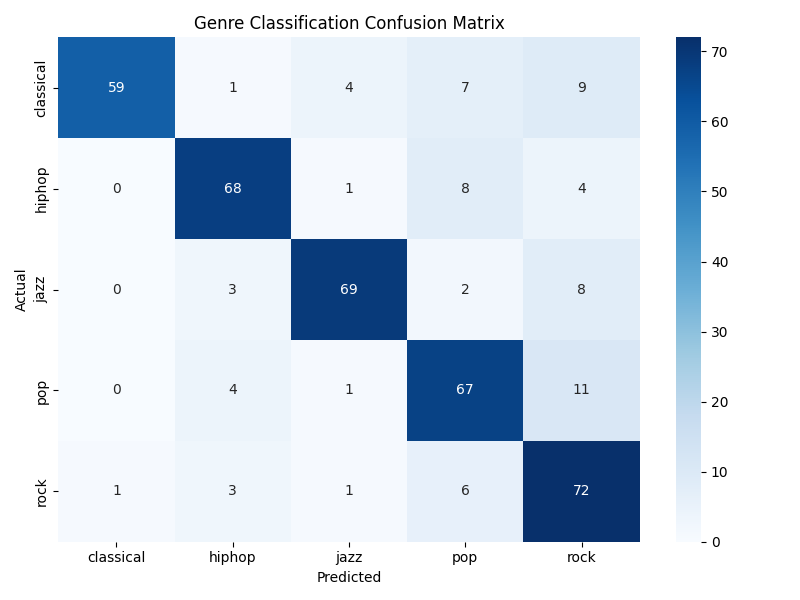
\includegraphics[width=0.88\textwidth]{genre_confusion_matrix.png}
\caption{Confusion matrix for genre classification.}
\label{fig:genrecm}
\end{figure}

The model performs well on structurally distinct genres such as Classical and Jazz, while moderate confusion is observed between Pop and Rock due to overlapping spectral characteristics.

\section{Emotion Recognition Results}

The Random Forest emotion recognition model achieved an overall accuracy of \textbf{92.61\%}. The classifier showed strong performance across all emotional categories.

\begin{table}[H]
\centering
\caption{Emotion Recognition Performance Metrics}
\label{tab:emotionmetrics}

\begin{tabular}{|c|c|c|c|}
\hline
\textbf{Emotion} & \textbf{Precision} & \textbf{Recall} & \textbf{F1-Score} \\
\hline
Angry & 0.90 & 0.97 & 0.93 \\
Calm & 0.94 & 0.95 & 0.95 \\
Happy & 0.94 & 0.82 & 0.88 \\
Sad & 0.92 & 0.94 & 0.93 \\
\hline
\end{tabular}

\end{table}

\begin{figure}[H]
\centering
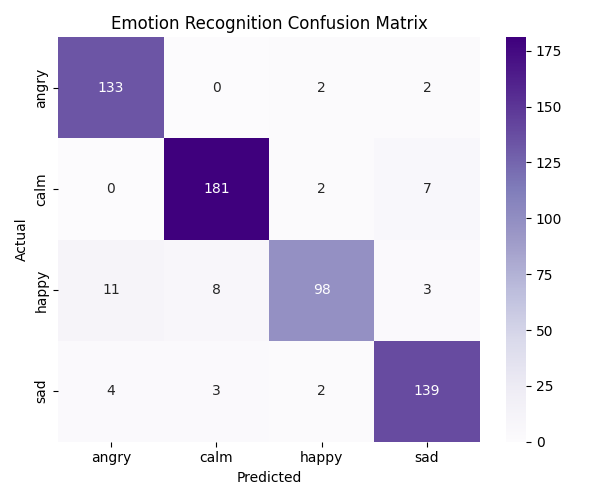
\includegraphics[width=0.84\textwidth]{emotion_confusion_matrix.png}
\caption{Confusion matrix for emotion recognition.}
\label{fig:emotioncm}
\end{figure}

Minor confusion is observed between Happy and Angry emotions because of similarities in tempo and energy characteristics across some music segments.

\section{Contextual Compatibility Analysis}

One of the key features of the framework is its ability to evaluate whether a music track matches the user’s current activity, mood, and desired mental state.

The contextual intelligence engine analyzes acoustic features, emotional behaviour, stimulation level, and semantic descriptors to generate compatibility scores and behavioral recommendations for activities such as studying, meditation, workouts, relaxation, and sleep preparation.

\begin{figure}[H]
\centering
\includegraphics[width=0.88\textwidth]{context_result.png}
\caption{Example output of contextual compatibility analysis.}
\label{fig:contextanalysis}
\end{figure}

The generated cognition metrics are heuristic indicators derived from acoustic and emotional characteristics and should not be interpreted as clinical psychological assessments.

\subsection{Visualization Outputs}

The framework also generates waveform plots, Mel-spectrograms, chromagrams, MFCC visualizations, emotion timelines, radar charts, and audio characteristic graphs to improve interpretability and transparency of predictions.

\section{Discussion}

The experimental results show that the framework can perform reliable music genre classification, emotion recognition, and contextual analysis in real time. The CNN successfully learns discriminative spectral patterns from Mel-spectrograms, while the Random Forest classifier effectively captures emotional behaviour using engineered acoustic features.

The integration of semantic profiling and contextual reasoning extends traditional music classification systems toward context-aware and emotionally adaptive music analysis \cite{r24,r27,r28}. Instead of only predicting labels, the system evaluates how suitable the music is for the user’s current context and cognitive requirements.

The framework also improves interpretability through explainable visualizations, behavioral analysis, and cognitive scoring. Current limitations include limited genre categories and the use of heuristic rule-based contextual reasoning instead of adaptive learning methods.

\section{Novel Contributions}

The system combines CNN-based genre classification, Random Forest-based emotion recognition, temporal emotion analysis, semantic profiling, contextual reasoning, cognition scoring, and explainable visualization within a single real-time framework.

Unlike conventional recommendation systems that rely mainly on metadata or listening history, this framework performs direct acoustic and behavioral analysis of music signals to estimate contextual suitability.

The project therefore moves beyond traditional genre prediction and establishes a foundation for context-aware cognitive music intelligence systems.

\chapter{TESTING AND DEPLOYMENT}

\section{System Testing}

The system was tested across multiple stages including audio preprocessing, genre classification, emotion recognition, contextual reasoning, visualization generation, and real-time Streamlit deployment.

Testing was performed using music tracks with different genres, emotional profiles, tempos, and acoustic structures. Uploaded audio files were successfully segmented, processed, and analyzed using both CNN-based and feature-based models.

The testing process verified audio upload, Mel-spectrogram generation, genre prediction, emotion timeline generation, contextual compatibility analysis, cognition scoring, and visualization rendering.

The framework showed stable behaviour across different audio durations and generated interpretable outputs with near real-time response during local execution.

\section{How to Run the Application}

The system is deployed as a Streamlit-based web application. To run the framework locally:

\begin{enumerate}

\item Install required dependencies:

\begin{verbatim}
pip install streamlit torch torchvision
pip install librosa matplotlib
pip install scikit-learn joblib
pip install numpy pandas pillow
\end{verbatim}

\item Ensure the project directory contains the trained models, preprocessing modules, datasets, and Streamlit application files.

\item Launch the application:

\begin{verbatim}
streamlit run app.py
\end{verbatim}

\item Upload an audio file in WAV or MP3 format and provide contextual inputs such as mood, activity, and desired outcome.

\item The system automatically performs preprocessing, feature extraction, prediction, contextual reasoning, and visualization generation before displaying the final outputs.

\end{enumerate}

\section{Deployment Workflow}

During inference, uploaded audio first passes through preprocessing stages including normalization, trimming, segmentation, and feature extraction.

The segmented audio is then processed through two parallel pipelines:
CNN-based genre classification using Mel-spectrograms and Random Forest-based emotion recognition using acoustic feature vectors.

The generated outputs are forwarded to the contextual intelligence engine, which creates semantic music profiles and evaluates compatibility with the user’s current emotional and cognitive state.

Final outputs including genre prediction, emotion analysis, compatibility scores, behavioral explanations, cognition metrics, and visualizations are displayed through the Streamlit dashboard.

\begin{figure}[H]
    \centering
    \includegraphics[width=0.9\textwidth]{deployment_workflow.png}
    \caption{Deployment workflow of the proposed music intelligence system.}
    \label{fig:deploymentworkflow}
\end{figure}

\section{Real-Time Inference Behaviour}

The framework performs near real-time inference on CPU-based systems with moderate computational requirements. Audio segmentation and feature extraction are efficiently handled using Librosa and NumPy, while the trained CNN and Random Forest models generate predictions with low latency.

Majority voting across segmented predictions improves robustness during genre classification, especially for longer music tracks containing local acoustic variations.

The system also dynamically generates waveform plots, spectrograms, MFCC visualizations, and emotion timelines during inference.

\section{Possible Improvements}

The current implementation can be further improved by using optimized deployment formats such as ONNX or TorchScript, GPU acceleration, larger datasets, adaptive contextual reasoning models, cloud deployment support, transformer-based audio architectures, and real-time streaming analysis.

Additional improvements may include multilingual voice interaction, personalized recommendation learning, and self-supervised audio representation models for better contextual understanding.

\chapter{CONCLUSION}

This project presents a context-aware audio intelligence system capable of performing music genre classification, emotion recognition, temporal emotion analysis, and cognitive compatibility evaluation using Artificial Intelligence techniques.

The system combines deep learning, machine learning, audio signal processing, contextual reasoning, and explainable AI within a real-time music analysis framework. The CNN model successfully learns discriminative spectral patterns from Mel-spectrogram representations, while the Random Forest classifier effectively captures emotional behaviour using acoustic features such as MFCCs, chroma features, tempo, spectral contrast, energy, and spectral descriptors.

Segment-wise audio analysis further improves robustness and enables temporal emotion tracking across music signals. Instead of only predicting static labels, the framework also evaluates whether a music track is suitable for the user’s current mood, activity, and desired mental state through semantic profiling and contextual reasoning.

The Streamlit-based application demonstrates the practical applicability of the system by providing real-time analysis, cognitive scoring, emotion timelines, behavioral interpretation, and explainable visualizations through an interactive interface.

Overall, the project shows how AI techniques can extend traditional music classification toward more human-centered and context-aware music analysis systems capable of supporting intelligent recommendation and adaptive listening experiences.

\addcontentsline{toc}{chapter}{Appendices}

\chapter*{Appendix}

\section*{A. Major Files in the Project}

\begin{itemize}

\item \texttt{app.py} --- Main Streamlit application.

\item \texttt{train\_model.py} --- CNN training pipeline for genre classification.

\item \texttt{predict.py} --- Genre prediction and majority voting.

\item \texttt{audio\_to\_img.py} --- Mel-spectrogram generation.

\item \texttt{generate\_images.py} --- Dataset image generation utility.

\item \texttt{audio\_feature.py} --- Acoustic feature extraction.

\item \texttt{train\_emodel.py} --- Emotion recognition model training.

\item \texttt{music\_profile.py} --- Semantic music profiling.

\item \texttt{compatibility\_rules.py} --- Contextual compatibility analysis.

\item \texttt{scores.py} --- Cognitive score generation.

\item \texttt{explain.py} --- Behavioral interpretation module.

\item \texttt{visualize.py} --- Audio visualization generation.

\item \texttt{model.pth} --- Trained CNN model.

\item \texttt{emotion\_model.pkl} --- Trained Random Forest model.

\end{itemize}

\section*{B. Key Commands}

\begin{verbatim}
python train_model.py
python train_emodel.py
streamlit run app.py
python generate_images.py
\end{verbatim}

\section*{C. Execution Environment}

\begin{itemize}

\item Python 3.10+

\item PyTorch and Torchvision --- CNN implementation

\item Scikit-learn --- Random Forest classification

\item Librosa --- Audio processing and feature extraction

\item Streamlit --- Web deployment

\item NumPy and Pandas --- Numerical computation

\item Matplotlib and Seaborn --- Visualization generation

\item Joblib --- Model serialization

\end{itemize}

\section*{D. Important Code Snippets}

\subsection*{CNN Genre Prediction}

\begin{lstlisting}
with torch.no_grad():

    outputs = model(image)

    probabilities = torch.softmax(
        outputs,
        dim=1
    )

    confidence, predicted = torch.max(
        probabilities,
        1
    )

genre = class_names[
    predicted.item()
]
\end{lstlisting}

\subsection*{Contextual Compatibility Analysis}

\begin{lstlisting}
context_result =
    analyze_music_context(

        feature_dict=feature_dict,
        emotions=emotions,
        emotion=overall_emotion,
        genre=genre,

        user_mood=user_mood,
        activity=activity,
        goal=goal
)
\end{lstlisting}

\subsection*{Temporal Emotion Analysis}

\begin{lstlisting}
for start in range(
        0,
        total_samples,
        chunk_samples
):

    end = start + chunk_samples

    chunk = y[start:end]

    feature_dict, feature_vector =
        extract_audio_features(
            y=chunk,
            sr=sr
        )

    pred = model.predict(
        [feature_vector]
    )[0]
\end{lstlisting}

\addcontentsline{toc}{chapter}{References}

\begin{thebibliography}{99}

\bibitem{r1}
G. Tzanetakis and P. Cook, ``Musical Genre Classification of Audio Signals,'' IEEE Transactions on Speech and Audio Processing, vol. 10, no. 5, pp. 293--302, 2002.

\bibitem{r2}
M. Müller and S. Ewert, ``Chroma Toolbox: MATLAB Implementations for Extracting Variants of Chroma-Based Audio Features,'' Proceedings of the International Society for Music Information Retrieval Conference (ISMIR), 2011.

\bibitem{r3}
K. Choi, G. Fazekas, and M. Sandler, ``Automatic Music Tagging Using Deep Convolutional Neural Networks,'' Proceedings of the International Society for Music Information Retrieval Conference (ISMIR), 2016.

\bibitem{r4}
S. Hershey et al., ``CNN Architectures for Large-Scale Audio Classification,'' Proceedings of the IEEE International Conference on Acoustics, Speech and Signal Processing (ICASSP), 2017.

\bibitem{r5}
J. Pons et al., ``Designing Efficient Architectures for Music Classification Using Convolutional Neural Networks,'' IEEE Access, vol. 7, pp. 128--139, 2019.

\bibitem{r6}
S. Dieleman and B. Schrauwen, ``End-to-End Learning for Music Audio,'' Proceedings of the IEEE International Conference on Acoustics, Speech and Signal Processing (ICASSP), 2014.

\bibitem{r7}
E. J. Humphrey, J. P. Bello, and Y. LeCun, ``Moving Beyond Feature Design in Music Informatics,'' Proceedings of the International Society for Music Information Retrieval Conference (ISMIR), 2012.

\bibitem{r8}
A. Kumar et al., ``Music Genre Classification Using Deep Neural Networks,'' Journal of Ambient Intelligence and Humanized Computing, vol. 12, no. 4, pp. 4543--4555, 2021.

\bibitem{r9}
Y. Liu et al., ``Hybrid CNN Model for Robust Music Genre Classification,'' Expert Systems with Applications, vol. 185, 2022.

\bibitem{r10}
A. Krizhevsky, I. Sutskever, and G. Hinton, ``ImageNet Classification with Deep Convolutional Neural Networks,'' Advances in Neural Information Processing Systems (NeurIPS), 2012.

\bibitem{r11}
D. Ellis, ``Chroma Feature Analysis and Synthesis,'' Columbia University Technical Report, 2007.

\bibitem{r12}
S. Choi, J. Kim, and K. Lee, ``Deep Chroma Feature Learning for Music Classification,'' IEEE Access, vol. 8, pp. 222342--222353, 2020.

\bibitem{r13}
Z. Fu et al., ``A Survey of Audio-Based Music Classification and Annotation,'' IEEE Transactions on Multimedia, vol. 13, no. 2, pp. 303--319, 2011.

\bibitem{r14}
H. Purwins et al., ``Deep Learning for Audio Signal Processing,'' IEEE Journal of Selected Topics in Signal Processing, vol. 13, no. 2, pp. 206--219, 2019.

\bibitem{r15}
F. Chollet, ``Deep Learning with Python,'' Manning Publications, 2018.

\bibitem{r16}
A. van den Oord et al., ``Representation Learning with Contrastive Predictive Coding,'' arXiv preprint arXiv:1807.03748, 2018.

\bibitem{r17}
T. Li and M. Ogihara, ``Music Genre Classification with Taxonomy,'' Proceedings of the IEEE International Conference on Multimedia and Expo (ICME), 2005.

\bibitem{r18}
K. Lee and D. Ellis, ``Audio-Based Semantic Concept Classification for Consumer Video,'' IEEE Transactions on Audio, Speech, and Language Processing, vol. 18, no. 6, pp. 1406--1416, 2010.

\bibitem{r19}
S. Marchand and G. Peeters, ``Scale-Invariant Audio Features for Musical Genre Classification,'' Proceedings of the International Conference on Digital Audio Effects (DAFX), 2016.

\bibitem{r20}
A. Paszke et al., ``PyTorch: An Imperative Style, High-Performance Deep Learning Library,'' Advances in Neural Information Processing Systems (NeurIPS), vol. 32, 2019.

\bibitem{r21}
Streamlit Inc., ``Streamlit Documentation,'' Available: https://docs.streamlit.io/, Accessed: 2026.

\bibitem{r22}
B. McFee et al., ``librosa: Audio and Music Signal Analysis in Python,'' Proceedings of the 14th Python in Science Conference, pp. 18--25, 2015.

\bibitem{r23}
L. Breiman, ``Random Forests,'' Machine Learning, vol. 45, no. 1, pp. 5--32, 2001.

\bibitem{r24}
J. Kang and D. Herremans, ``Are We There Yet? A Brief Survey of Music Emotion Prediction Datasets, Models and Outstanding Challenges,'' arXiv preprint arXiv:2406.08809, 2024.

\bibitem{r25}
X. Jiang et al., ``Music Emotion Recognition Based on Deep Learning: A Review,'' IEEE Access, vol. 12, pp. 157716--157744, 2024.

\bibitem{r26}
Y. Wang et al., ``A Survey on Music Emotion Recognition Using Learning Models,'' Multimedia Systems, vol. 31, no. 278, 2025.

\bibitem{r27}
P. L. Louro et al., ``A Comparison Study of Deep Learning Methodologies for Music Emotion Recognition,'' Sensors, vol. 24, no. 7, 2024.

\bibitem{r28}
Y. Sun et al., ``Feature Centric Based Deep Learning Approach for Music Mood Classification,'' Scientific Reports, vol. 15, 2025.

\end{thebibliography}


\end{document}